%! TEX root = main.tex

\graphicspath{{00_Images/11_chapter/}}

\chapter{Introduction to Microphones and Specifications}
\label{ch:microphone_intro}

A microphone is an electroacoustic transducer that converts acoustic pressure variations in the surrounding sound field into a corresponding electrical voltage at its output terminals.
In this sense it performs the inverse function of the electrodynamic loudspeaker studied in the preceding chapters: rather than driving a diaphragm to radiate sound, the microphone senses the mechanical displacement imposed on a diaphragm by an incoming wave and delivers an electrical signal proportional to the sound pressure.
Microphones are classified along three independent axes.
According to the transduction principle, the main families are condenser (capacitor), moving-coil (dynamic) and piezoelectric (crystal) types.
According to function, a microphone may be designed for calibrated sound-level measurement, for speech or sound reinforcement or for studio and recording applications.
According to directional characteristic, the sensitivity pattern can be omnidirectional, cardioid, supercardioid or hypercardioid, depending on how the capsule is exposed to the sound field.
This chapter presents the principal transduction mechanisms, defines the key performance parameters, sensitivity, noise, dynamic range and frequency response and provides an overview of directional behavior that will be developed quantitatively in the chapters that follow.

\section{Transduction Principles}
\label{sc:111}

The history of the microphone spans roughly a century of progressive refinement, beginning with electrochemical and electromagnetic techniques and culminating in the precision capacitive transducers that dominate modern studio and measurement practice.
The following survey introduces each mechanism at the level of detail needed to understand why condenser and moving-coil types have displaced the earlier designs and how the underlying physics shapes the practical characteristics of each family.

\subsection{Historical Types}

\paragraph{Carbon microphone} The carbon microphone, introduced commercially by Westinghouse around 1921, operates on a piezoresistive principle.
A metallic diaphragm is pressed against a cup filled with carbon granules; acoustic pressure deforms the diaphragm, compressing or expanding the granule bed and thereby changing the electrical resistance of the medium.
A DC voltage applied across the element converts this resistance variation into a current signal, which is then stepped up in voltage by a series transformer that simultaneously performs AC coupling and impedance transformation to the load.
Despite its historical importance as the dominant telephone transducer for several decades, the carbon microphone suffers from high self-noise, strong nonlinear distortion and a frequency response that rolls off markedly above a few kilohertz and it has been completely superseded in all audio applications.

\paragraph{Ribbon microphone} The ribbon microphone, developed around 1933, suspends a thin corrugated metallic ribbon in the gap of a permanent magnet.
Incident sound waves set the ribbon into velocity-proportional vibration and, by Faraday's induction law, a voltage proportional to the ribbon velocity is induced along its length.
Because the ribbon element is intrinsically a low-impedance, low-voltage source, a step-up transformer is mounted directly behind it to deliver a usable signal level to the preamplifier.
The ribbon microphone exhibits a natural figure-eight (bidirectional) polar pattern, an extended and smooth frequency response and a characteristic warm tonal quality valued for orchestral and vocal recording; its practical limitations are mechanical fragility and sensitivity lower than that of condenser types.

\paragraph{Crystal microphone} The crystal or piezoelectric, microphone relies on the direct piezoelectric effect: mechanical deformation of a crystalline material generates an electric charge across its faces.
Sound waves displace a lightweight diaphragm that presses against a piezoelectric element, producing an output voltage proportional to the applied pressure.
Crystal microphones are mechanically simple and inexpensive, but they exhibit high output impedance, limited frequency range and poor environmental stability, making them unsuitable for professional applications.

\subsection{Moving-Coil Microphone}

The moving-coil microphone, also called the dynamic microphone, operates on the same electromagnetic principle as the electrodynamic loudspeaker, but with the direction of energy conversion reversed.
A lightweight diaphragm, typically fabricated from a polyester film such as Mylar, is mechanically coupled to a cylindrical coil of fine wire wound around a former that sits in the annular gap of a permanent magnet.
Incident acoustic pressure displaces the diaphragm, which carries the coil axially through the static magnetic field; by the Lorentz law applied in reverse, this motion induces an electromotive force across the coil terminals proportional to the coil velocity:
\[
v_{\mathrm{out}} = B l u_c
\]
where \(B\) is the magnetic flux density in the gap, \(l\) is the total effective length of wire immersed in the field and \(u_c\) is the instantaneous coil velocity.
Because the moving-coil capsule is sensitive to external low-frequency magnetic interference such as that produced by power-line transformers, a compensating hum-bucking coil wound in opposition is commonly incorporated to cancel the induced interference.
Moving-coil microphones require no polarization voltage, tolerate high sound pressure levels without distortion and are mechanically robust against rough handling and adverse environmental conditions, making them the standard choice for live sound reinforcement and broadcast applications.

\subsection{Condenser Microphone}

The condenser (capacitor) microphone represents the most accurate and most widely used transduction principle in both professional recording and precision measurement.
Its capsule consists of two electrically conductive elements separated by a narrow air gap of approximately \SIrange{15}{30}{\micro\meter}: a thin, tensioned metallic diaphragm exposed to the sound field and a fixed, perforated backplate.
Together they form a capacitor with capacitance:
\[
C = \varepsilon \frac{A}{d}
\]
where \(\varepsilon\) is the permittivity of air, \(A\) is the effective electrode area and \(d\) is the gap distance.

\begin{figure}[!htb]
    \centering
    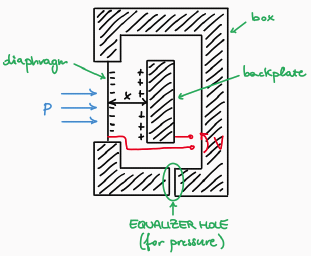
\includegraphics[width=0.45\textwidth]{condenser_mic.png}
    \caption{Cross-section of a condenser microphone capsule showing the tensioned diaphragm, the \SIrange{15}{30}{\micro\meter} air gap and the perforated backplate}
\end{figure}

The capsule is held at a constant charge \(Q\) by a high-impedance DC bias circuit, so that the capacitor law \(Q = C V\) implies:
\[
\Delta V \approx -V_B \frac{\Delta C}{C_0} \approx V_B \frac{\Delta d}{d_0}
\]
where \(V_B\) is the bias voltage, \(C_0\) is the equilibrium capacitance and \(d_0\) is the equilibrium gap.
The output voltage is therefore directly proportional to the diaphragm displacement and since that displacement is proportional to acoustic pressure in the stiffness-controlled regime, the transduction chain is linear: \(v_{\mathrm{out}} \propto p\).
A standard bias of \SI{48}{\volt} (phantom power) is supplied symmetrically through the balanced XLR cable and used to polarize the capsule and power the internal impedance-converter circuitry.
The condenser principle offers lower noise, wider frequency range and higher sensitivity than all other transduction types; its only practical requirements are a stable bias supply and careful management of humidity, since the very high bias impedance renders the capsule susceptible to surface contamination.

\section{Sensitivity and Sound Pressure Level}
\label{sc:112}

\subsection{Sensitivity Definition}

The sensitivity \(S\) of a microphone is the fundamental figure of merit that quantifies how efficiently acoustic pressure is converted into an electrical voltage at the output terminals.
It is defined as the ratio of the open-circuit output voltage \(v_{\mathrm{out}}\) to the incident sound pressure \(p\), measured at a specified reference frequency (conventionally \SI{1}{\kilo\hertz}) under free-field conditions with the wave arriving on-axis:
\[
S = \frac{v_{\mathrm{out}}}{p} \quad \left[\si{\volt\per\pascal}\right]
\]
A typical value for a professional condenser microphone is \(S = \SI{10}{\milli\volt\per\pascal}\).
Because the sensitivity spans many orders of magnitude across different microphone classes, it is more conveniently expressed in decibels relative to the standard reference value \(S_{\mathrm{REF}} = \SI{1}{\volt\per\pascal}\):
\[
S_{\mathrm{dB}} = 20\log_{10}\left(\frac{S}{S_{\mathrm{REF}}}\right)
\]
Some representative values and their decibel equivalents are listed below:
\begin{itemize}
    \item \SI{1}{\volt\per\pascal} \(\to\) \(\SI{0}{\decibel} \mathrm{V/Pa}\)
    \item \SI{100}{\milli\volt\per\pascal} \(\to\) \(-20 \mathrm{dB} \mathrm{V/Pa}\)
    \item \SI{10}{\milli\volt\per\pascal} \(\to\) \(-40 \mathrm{dB} \mathrm{V/Pa}\)
    \item \SI{1}{\milli\volt\per\pascal} \(\to\) \(-60 \mathrm{dB} \mathrm{V/Pa}\)
    \item \SI{100}{\micro\volt\per\pascal} \(\to\) \(-80 \mathrm{dB} \mathrm{V/Pa}\)
\end{itemize}

\subsection{Sound Pressure Level}

The sound pressure level (SPL) is defined as:
\[
\mathrm{SPL} = 20\log_{10}\left(\frac{p_{\mathrm{RMS}}}{p_{\mathrm{ref}}}\right) \quad [\mathrm{dB SPL}]
\]
where the reference pressure \(p_{\mathrm{ref}} = \SI{20}{\micro\pascal}\) corresponds to the threshold of hearing at \SI{1}{\kilo\hertz} for a young person with normal hearing and defines the \SI{0}{\decibel} point of the SPL scale.
The acoustic domain of interest for audio applications spans from \SI{0}{\decibel SPL} (threshold of audibility, \(\approx \SI{20}{\micro\pascal}\)) to approximately \SI{140}{\decibel SPL} (threshold of pain, \(\approx \SI{200}{\pascal}\)), covering seven decades of absolute pressure.
Since the microphone output voltage is proportional to pressure through the sensitivity, any position on the SPL axis maps directly to a corresponding output voltage: for \(S = \SI{10}{\milli\volt\per\pascal}\), a conversation at \SI{60}{\decibel SPL} produces roughly \SI{20}{\milli\pascal} and thus \(\SI{0.2}{\milli\volt}\) at the microphone output, while a nearby jackhammer at \SI{100}{\decibel SPL} produces \SI{2}{\pascal} and \SI{20}{\milli\volt}.

\subsection{Specification Example: Shure KSM9}

The Shure KSM9 electret condenser microphone illustrates how the sensitivity specification is applied in practice.
Its data sheet lists:
\begin{itemize}
    \item Sensitivity (open-circuit, at \SI{1}{\kilo\hertz}): \(-51 \mathrm{dBV/Pa}\), equivalent to \(\SI{2.8}{\milli\volt\per\pascal}\)
    \item Maximum SPL at \SI{1}{\percent} THD: \SI{152}{\decibel SPL}
    \item Self-noise: \SI{22}{\decibel SPL} (A-weighted)
    \item Dynamic range: \SI{130}{\decibel}
\end{itemize}
The maximum SPL corresponds to an acoustic pressure of:
\[
p_{\mathrm{max}} = \SI{20}{\micro\pascal} \times 10^{152/20} \approx \SI{796}{\pascal}
\]
yielding a peak output voltage of:
\[
v_{\mathrm{out,max}} = S \times p_{\mathrm{max}} = \SI{2.8}{\milli\volt\per\pascal} \times \SI{796}{\pascal} \approx \SI{2.2}{\volt}
\]
This figure sets the clipping level that the preamplifier input stage must accommodate without distortion.
Conversely, at a quiet conversational SPL of \SI{60}{\decibel SPL} the output is only \SI{0.06}{\milli\volt}, illustrating the enormous dynamic range the downstream electronics must handle, from microvolts to volts within the same system.

\section{Directionality}
\label{sc:113}

\subsection{Directional Sensitivity}

The sensitivity of a microphone depends in general on the direction from which the sound arrives.
This angular dependence is characterized by the relative directional sensitivity function:
\[
S_{\mathrm{REL}}(\alpha) = \frac{S(\alpha)}{S(0)}
\]
where \(\alpha\) is the angle of incidence measured from the diaphragm normal axis and \(S(0)\) is the on-axis sensitivity.
Expressed in decibels:
\[
S_{\mathrm{REL},\mathrm{dB}}(\alpha) = 20\log_{10}\left(\frac{S(\alpha)}{S(0)}\right)
\]
Since the on-axis direction \(\alpha = 0\) typically corresponds to maximum sensitivity, \(S_{\mathrm{REL}}(\alpha) \leq 1\) and \(S_{\mathrm{REL},\mathrm{dB}}(\alpha) \leq 0 \mathrm{dB}\) for all other angles.
The complete angular dependence is displayed as a polar pattern, which plots \(S_{\mathrm{REL},\mathrm{dB}}(\alpha)\) in polar coordinates on concentric reference circles conventionally spaced at \SI{5}{\decibel} or \SI{10}{\decibel} intervals.

\subsection{Polar Pattern Types}

The principal directional characteristics encountered in practice are shown in figure \ref{fig:polarPatterns}.

\begin{figure}[!htb]
    \centering
    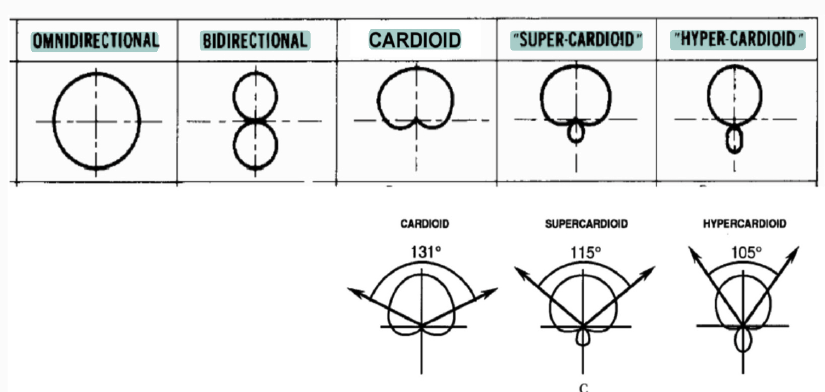
\includegraphics[width=0.80\textwidth]{directivity_pattern.png}
    \caption{Principal microphone polar patterns: omnidirectional, cardioid, supercardioid, hypercardioid and bidirectional (figure-eight)}
    \label{fig:polarPatterns}
\end{figure}

An omnidirectional microphone responds equally to sound from all directions (\(S_{\mathrm{REL}}(\alpha) = 1\) for all \(\alpha\)), while a bidirectional (figure-eight) microphone responds equally from the front and rear but exhibits a null at the sides (\(\alpha = 90°\)).
Intermediate patterns, obtained by combining pressure and pressure-gradient sensing as analyzed in the following chapter, yield the cardioid, supercardioid and hypercardioid families.
The cardioid exhibits a null at \(\alpha = 180°\), while the supercardioid and hypercardioid achieve a narrower main lobe at the expense of a small rear lobe.
Because of their forward-oriented pickup, directional microphones offer a higher ratio of on-axis to ambient response than the omnidirectional pattern: at equal working distance, a cardioid rejects diffuse ambient sound approximately \SI{4.8}{\decibel} more effectively than an omnidirectional microphone, a supercardioid provides \SI{5.8}{\decibel} more rejection and a hypercardioid provides \SI{6}{\decibel} more.
Equivalently, a cardioid may be placed approximately \(1.7\) times farther from the source than an omnidirectional microphone while maintaining the same signal-to-ambient ratio, a supercardioid at \(1.9\) times and a hypercardioid at \(2\) times.

\subsection{Omnidirectional Microphones}

Omnidirectionality is achieved by exposing the diaphragm to the sound field exclusively through a single front entry, so that the rear of the diaphragm is enclosed in a sealed cavity at ambient pressure.
At low frequencies, where the acoustic wavelength \(\lambda\) greatly exceeds the microphone body diameter \(D\), diffraction wraps the wave around the body and the capsule acts as a point obstacle: the pressure field reaches the diaphragm with essentially the same amplitude regardless of the direction of incidence and the response is genuinely omnidirectional.
At high frequencies, when \(\lambda\) becomes comparable to \(D\), the microphone body casts an acoustic shadow on the rear face of the capsule and the response becomes strongly direction-dependent.
The condition for omnidirectional behavior at a given frequency is therefore:
\[
\lambda > 10 D \quad \Longrightarrow \quad f < \frac{c}{10 D} \approx \frac{3}{D [\mathrm{cm}]} \mathrm{kHz}
\]
A capsule intended to remain omnidirectional up to \SI{20}{\kilo\hertz} must have a diaphragm diameter no larger than approximately \SI{1.7}{\milli\meter}; a standard half-inch (\SI{12.7}{\milli\meter}) capsule begins to exhibit directional narrowing above roughly \SI{2.4}{\kilo\hertz}.

\begin{figure}[!htb]
    \centering
    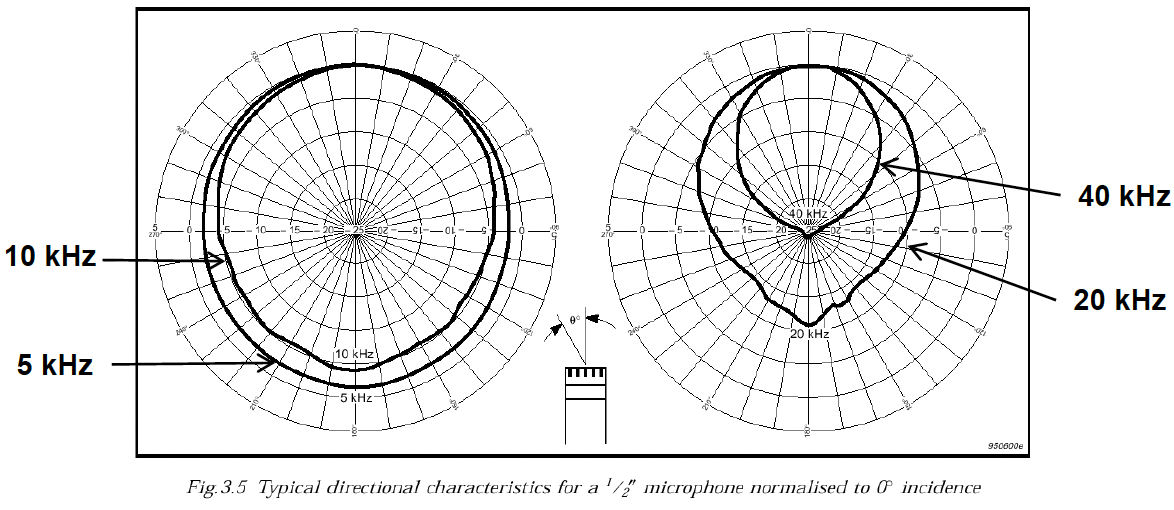
\includegraphics[width=0.70\textwidth]{omni_mic.png}
    \caption{Directional characteristics of a \(\tfrac{1}{2}''\) omnidirectional microphone normalized to \(0°\) incidence, showing the progressive departure from omnidirectionality as frequency increases from \SI{5}{\kilo\hertz} to \SI{40}{\kilo\hertz}: the acoustic shadow effect confines the effective pickup angle as \(\lambda\) approaches \(D\)}
\end{figure}

\subsection{Directional Microphones}

Directional microphones achieve their pattern by providing acoustic access to both the front and the rear of the diaphragm through multiple entries.
The rear entry is connected to the diaphragm through an internal acoustic path that introduces a delay of approximately one half-period at the design frequency, so that the rear wave arrives out of phase with the front wave.
For sound arriving from the front (\(\alpha = 0°\)), the front wave and the phase-shifted rear wave reinforce each other in displacing the diaphragm, producing maximum sensitivity.
For sound arriving from the rear (\(\alpha = 180°\)), both sides of the diaphragm receive the same wave simultaneously, so the two contributions cancel and the net diaphragm displacement is zero.

\begin{figure}[!htb]
    \centering
    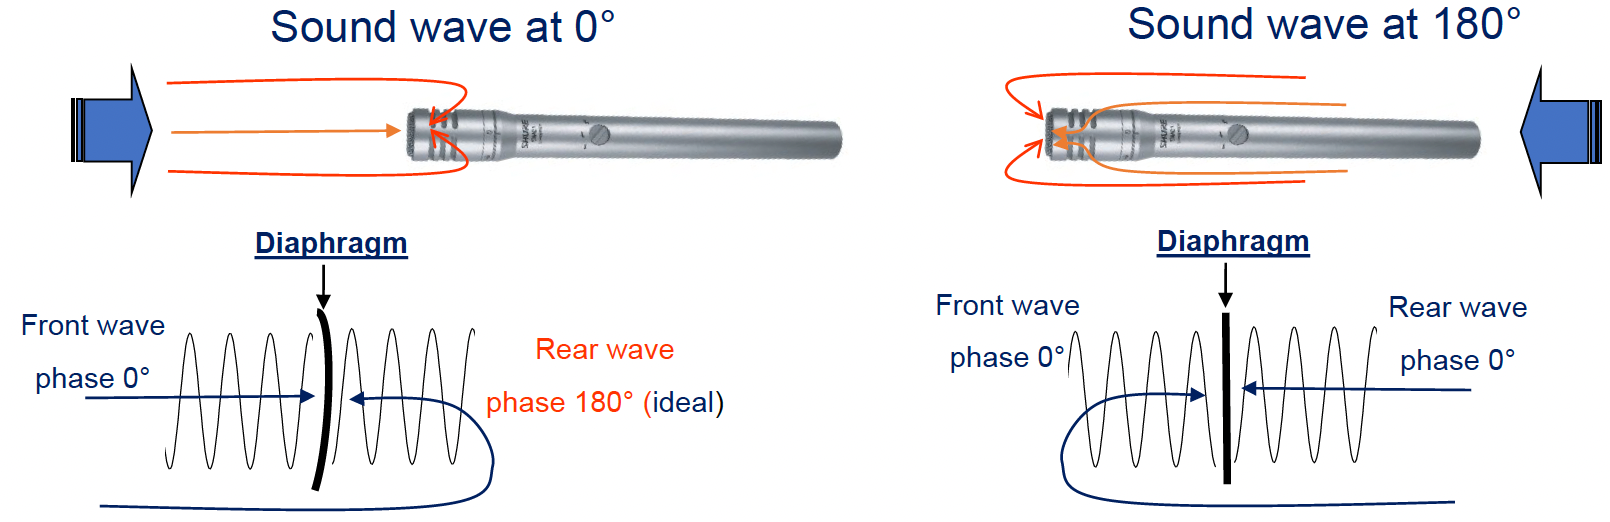
\includegraphics[width=0.80\textwidth]{directional_mic.png}
    \caption{Operating principle of a directional microphone with front and rear acoustic entries: a wave arriving at \(0°\) drives the diaphragm coherently through the delayed rear path (left), while a wave arriving at \(180°\) reaches both faces simultaneously and produces cancellation (right)}
\end{figure}

Some high-performance condenser microphones incorporate two diaphragms oriented in opposite directions and sharing a common backplate.
By varying the relative bias voltages applied to the two capsule halves, the polar pattern is adjusted continuously from omnidirectional through wide-angle cardioid, cardioid, hypercardioid and bidirectional, without any mechanical modification of the capsule.
The directionality in a real acoustic environment may differ substantially from the free-field polar pattern: nearby reflecting surfaces, including a human head positioned close to the microphone, scatter and redirect sound so that energy nominally arriving from the rear reaches the diaphragm from other directions, partially reducing the intended rear rejection.

\begin{figure}[!htb]
    \centering
    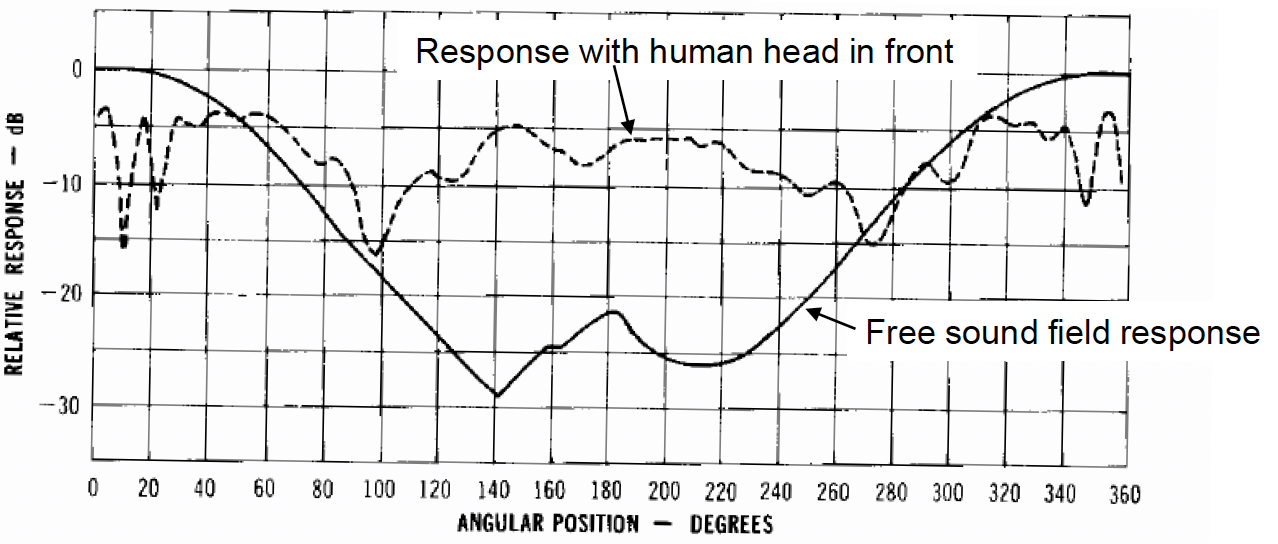
\includegraphics[width=0.70\textwidth]{obstacle_consequence.png}
    \caption{Effect of a nearby head obstacle on the effective polar response of a cardioid microphone: mid-frequency reflections off the head partially fill the rear null, illustrated by the dashed curve compared to the free-field response (solid curve)}
\end{figure}

\subsection{Highly Directional Microphones}

When the working distance between source and microphone is large, the sound pressure at the capsule drops significantly, requiring increased preamplifier gain, which simultaneously raises the captured level of diffuse ambient noise.
Interference-tube microphones (commonly called shotgun microphones) address this problem by placing a long tube of \SIrange{20}{40}{\centi\meter} with multiple lateral apertures in front of a directional capsule.
Off-axis sound waves enter the tube at multiple apertures spaced along its length and travel different distances to the diaphragm, accumulating phase shifts that produce destructive interference; on-axis sound waves travel directly to the far end of the tube and are captured coherently.
The resulting polar pattern is considerably narrower than a standard cardioid, enabling precise aiming at a distant source with strong rejection of off-axis and ambient contributions.

\begin{figure}[!htb]
    \centering
    \subfloat[Polar pattern of the Sennheiser MKH416 shotgun microphone]{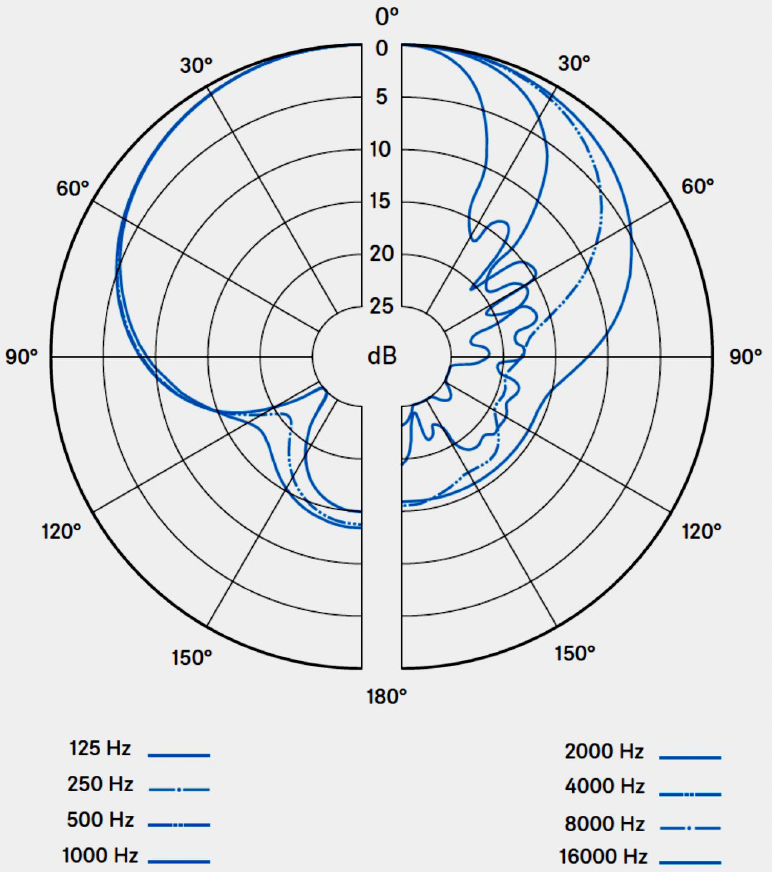
\includegraphics[width=0.33\linewidth]{highly_directional_mic.png}}
    \hfill
    \subfloat[Principle of the interference-tube assembly]{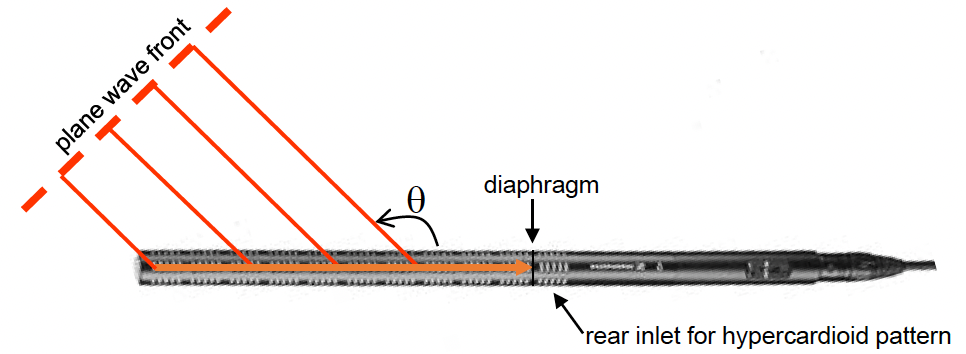
\includegraphics[height=0.15\textheight]{shotgun_mic_view.png}}
    \caption{Highly directional (shotgun) microphone: the interference tube narrows the main lobe strongly above the frequency at which the tube length exceeds half a wavelength, while a rear hypercardioid port maintains some rear rejection at low frequencies}
\end{figure}

\section{Frequency Response and Proximity Effect}
\label{sc:114}

\subsection{Relative Frequency Response}

The frequency response of a microphone quantifies how its sensitivity varies with the frequency of the incident sound.
It is defined as the relative sensitivity referred to the on-axis value at \SI{1}{\kilo\hertz}:
\[
S_{\mathrm{rel}}(f) = 20\log_{10}\left(\frac{S(f)}{S(\SI{1}{\kilo\hertz})}\right) \quad [\mathrm{dB}]
\]
An ideal microphone would exhibit \(S_{\mathrm{rel}}(f) = 0 \mathrm{dB}\) across the entire audio band from \SI{20}{\hertz} to \SI{20}{\kilo\hertz}, meaning that sensitivity is independent of frequency.
In practice, the response is bounded at the low end by the time constant of the static pressure equalization vent, which defines a high-pass cutoff below which the capsule ceases to respond to slowly varying pressure differences and at the high end by the finite relationship between the diaphragm diameter and the acoustic wavelength.

\subsection{Influence of Diaphragm Diameter}

The diaphragm diameter \(D\) governs a fundamental trade-off between sensitivity and upper frequency limit.
The sensitivity is proportional to the square of the diameter:
\[
S \propto D^2
\]
while the upper frequency at which a flat response is maintained is approximately inversely proportional to \(D\):
\[
f_{\mathrm{high}} \propto \frac{1}{D}
\]
A large diaphragm therefore delivers high sensitivity but a restricted high-frequency bandwidth, while a small diaphragm extends the flat band at the cost of reduced sensitivity.
Microphones of the same nominal diaphragm size can exhibit different sensitivities depending on the tension applied to the diaphragm during fabrication: lower tension increases mechanical compliance and raises sensitivity, while higher tension raises the resonance frequency and extends the high-frequency response.

\begin{figure}[!htb]
    \centering
    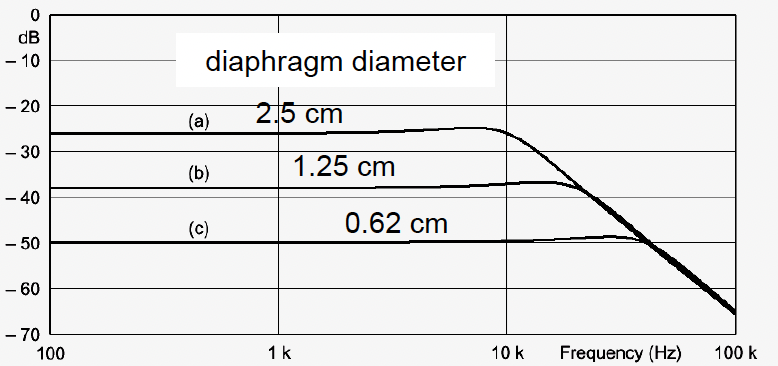
\includegraphics[width=0.65\textwidth]{diaphragm_diameter.png}
    \caption{Calculated frequency response magnitude for condenser capsules with diaphragm diameters of \SI{2.5}{\centi\meter}, \SI{1.25}{\centi\meter} and \SI{0.62}{\centi\meter} (curves a, b, c respectively): the flat band extends to progressively higher frequencies as the diaphragm is made smaller, at the expense of lower absolute sensitivity}
\end{figure}

\subsection{Proximity Effect}

Directional microphones, which sense the pressure difference across the two faces of the diaphragm, exhibit a characteristic low-frequency boost when the sound source is brought very close to the capsule.
This effect arises because the pressure gradient in the near field of a point source contains an additional \(1/r^2\) term beyond the far-field \(1/r\) contribution; at close distances this near-field gradient term becomes dominant and enhances the differential pressure driving the diaphragm at low frequencies, where the inter-face path difference constitutes a larger fraction of the wavelength.
The physical modeling of this mechanism is developed in detail in the following chapter; at this stage it suffices to note its practical consequence: as the source-to-microphone distance decreases below approximately \SI{30}{\centi\meter}, the low-frequency response rises progressively, producing a bass emphasis that grows more pronounced as the microphone is brought closer to the source.

\begin{figure}[!htb]
    \centering
    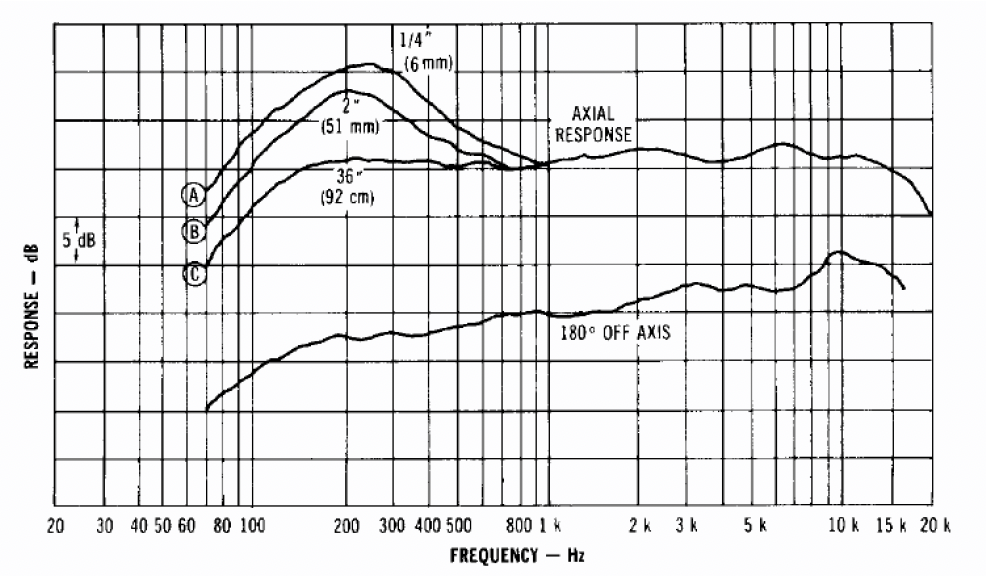
\includegraphics[width=0.65\textwidth]{proximity_effect.png}
    \caption{Position-dependent frequency response of a single-entry cardioid condenser microphone: the low-frequency response rises by several decibels as the source-to-microphone distance decreases from \SI{30}{\centi\meter} to \SI{7.5}{\centi\meter}, demonstrating the proximity effect}
\end{figure}

Many directional microphones intended for close-range vocal use are deliberately designed with a rolled-off low-frequency response at large distances, relying on the proximity effect to restore low-frequency energy when used close in, thereby achieving a balanced overall timbre.
In applications where proximity-effect coloration is undesirable, an internally switchable high-pass filter (often implementing a \SI{-6}{\decibel\per\octave} slope with a cutoff between \SI{80}{\hertz} and \SI{160}{\hertz}) allows the user to compensate.

\subsection{Static Pressure Equalization}

The static atmospheric pressure varies slowly over time due to weather changes and altitude differences at the recording site.
Even a change of \SI{1}{\milli\bar} corresponds to \SI{100}{\pascal}, a pressure \(10^8\) to \(10^9\) times larger than the faintest sound pressures to be captured; without compensation, such variations would displace the diaphragm far from its nominal rest position and fundamentally alter the capsule operating point.
To prevent this, every condenser capsule is equipped with a static pressure equalization vent, a narrow air channel connecting the internal cavity to the external atmosphere.
The vent allows the mean internal pressure to track the environmental static pressure with a time constant \(\tau\) set by the acoustic resistance and compliance of the channel, while leaving the acoustic signal band unaffected; the resulting low-frequency cutoff is:
\[
f_p = \frac{1}{2\pi \tau}
\]
For measurement microphones the time constant is typically \SI{0.1}{\second}, corresponding to a cutoff at approximately \SI{1.6}{\hertz}, which ensures a flat magnitude response down to below \SI{5}{\hertz} while filtering out all atmospheric drift.

\begin{figure}[!htb]
    \centering
    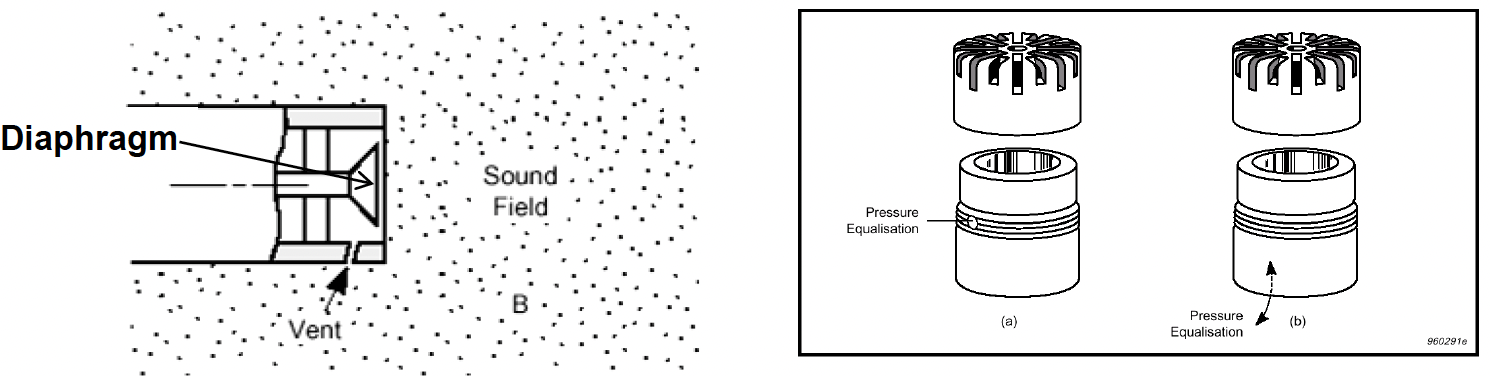
\includegraphics[width=0.65\textwidth]{mic_vent.png}
    \caption{Static pressure equalization vent in an omnidirectional condenser capsule: the narrow air channel (labeled B in the cross-section) connects the sealed rear cavity to the external atmosphere, allowing slow static pressure equalization while leaving the audio-band response unaffected}
\end{figure}

\subsection{Wind Noise and Protection}

Air flow across the microphone capsule generates turbulent pressure fluctuations at the diaphragm surface that are transduced as broadband noise, degrading the signal-to-noise ratio particularly at low frequencies.
This wind noise is distinct from acoustic noise in the sound field: it arises from the local aerodynamic boundary layer and is therefore not reproduced by headphone monitoring of a recording made simultaneously at a different position.
Three types of protection are commonly employed in practice: an internal wire-mesh windscreen integrated into the microphone grille, an external foam polyurethane slip-on windscreen that increases the effective turbulence distance from the diaphragm and an external pop filter (a stretched fabric membrane on a ring mount) positioned between the sound source and the microphone specifically to attenuate low-frequency plosive bursts from vocalists.

\begin{figure}[!htb]
    \centering
    \subfloat[Wind noise versus wind speed for windscreens of different diameters]{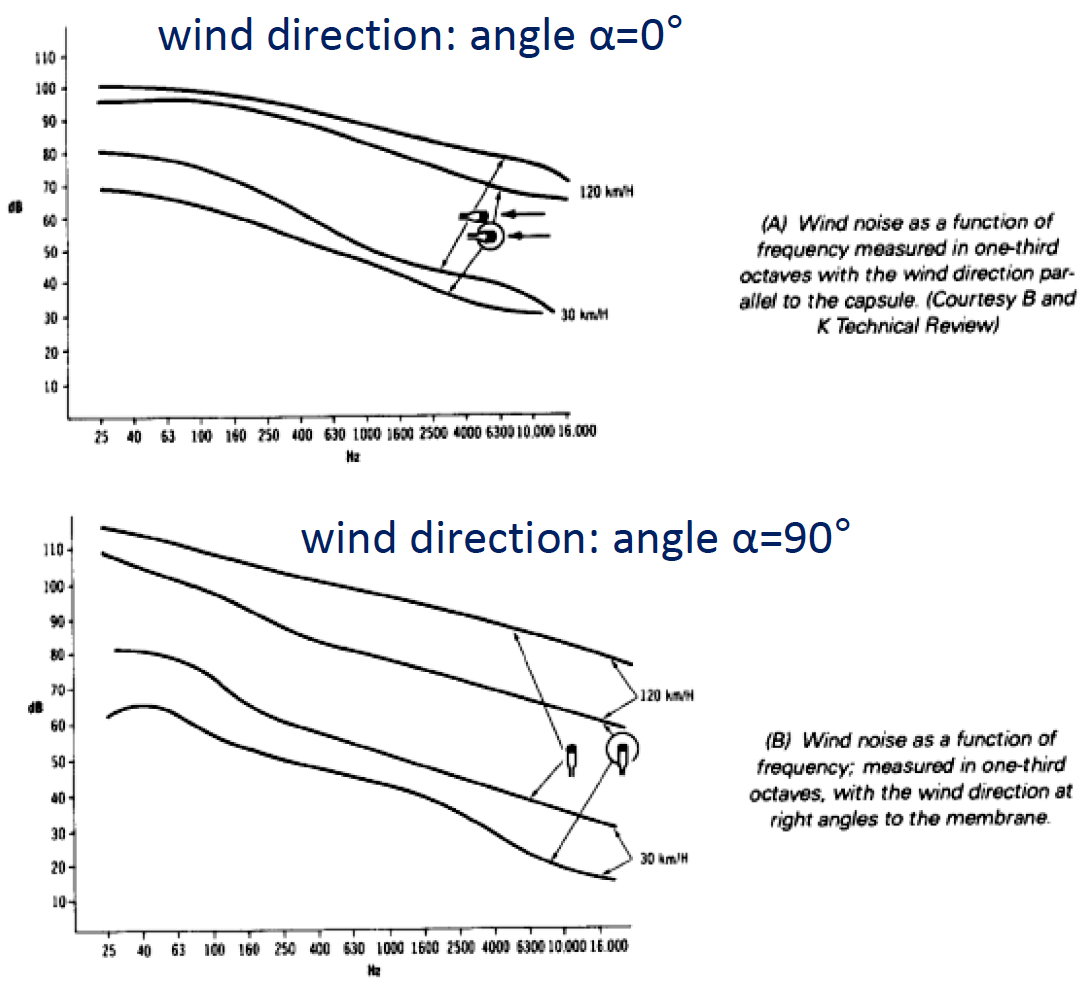
\includegraphics[height=0.25\textheight]{wind_noise_measurment.png}}
    \hfill
    \subfloat[Wind noise spectra at two wind directions]{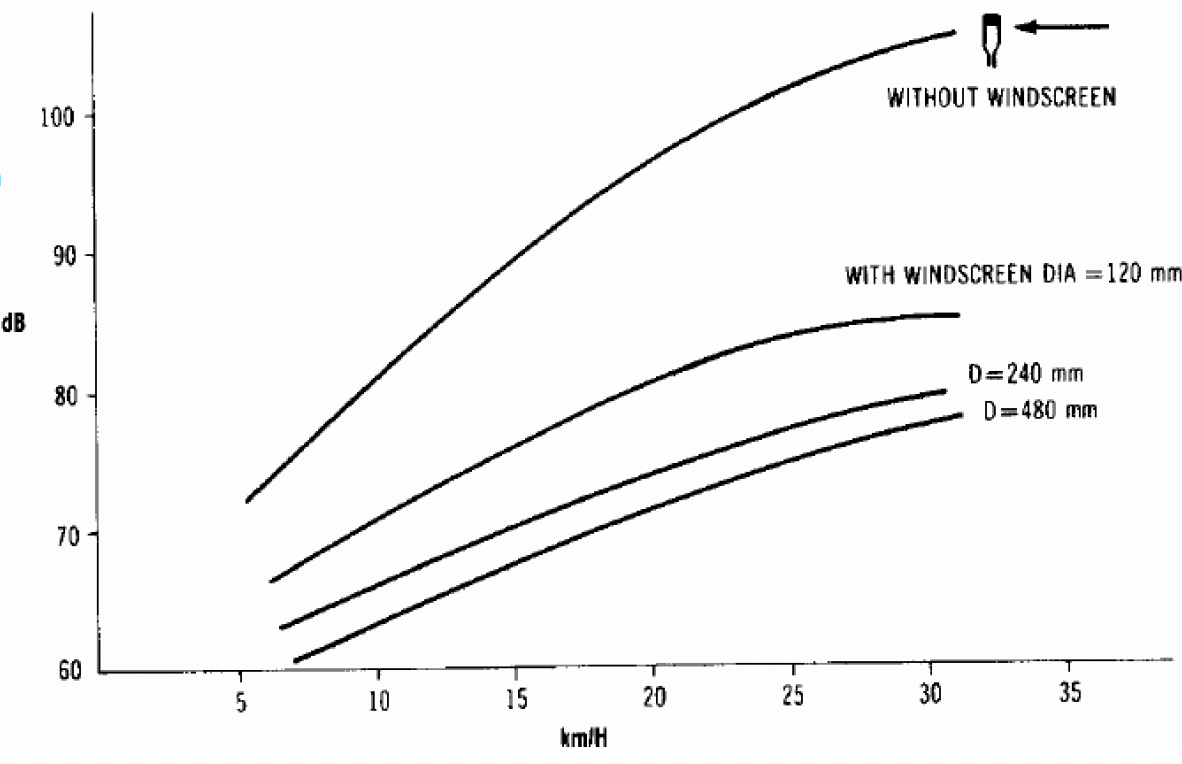
\includegraphics[height=0.25\textheight]{wind_noise.png}}
    \caption{Effect of windscreens on microphone noise: a larger windscreen body reduces turbulence-induced noise at a given wind speed, but all protection devices introduce some attenuation of the high-frequency signal response}
\end{figure}

\section{Noise and Dynamic Range}
\label{sc:115}

\subsection{Thermal Noise of the Microphone}

Even in a perfectly quiet acoustic environment, the microphone diaphragm is never at rest.
The thermal agitation of air molecules at finite temperature produces a continuous random bombardment of the diaphragm surface, inducing microscopic random displacements known as Brownian motion; these displacements are transduced into a fluctuating output voltage at the microphone terminals in the complete absence of any sound stimulus and constitute the irreducible lower limit of detectable acoustic pressure.
The noise voltage at the output can be referred back to the acoustic domain through the microphone sensitivity:
\[
p_{\mathrm{noise}} [\si{\pascal}_{\mathrm{RMS}}] = \frac{v_{\mathrm{noise}} [\si{\volt}_{\mathrm{RMS}}]}{S [\si{\volt\per\pascal}]}
\]
The resulting noise level is expressed in decibels relative to the standard reference pressure:
\[
\text{Noise level [dB SPL]} = 20\log_{10}\left(\frac{p_{\mathrm{noise}}}{\SI{20}{\micro\pascal}}\right)
\]
Typical self-noise values range from approximately \SI{0}{\decibel SPL} for large-diaphragm measurement-grade capsules to \SI{40}{\decibel SPL} for small-diaphragm designs.
For a condenser capsule, the noise pressure power spectral density is governed by the diaphragm mechanical parameters:
\[
\frac{\mathrm{d}P^2}{\mathrm{d}f} = 4kT \frac{2 \sigma t}{\pi R^4}
\]
where \(k\) is Boltzmann's constant, \(T\) is the absolute temperature, \(R\) is the diaphragm radius and \(\sigma t\) is the diaphragm tension per unit width.
Since the capsule sensitivity scales as \(R^2 / (\sigma t)\), the same design parameters that maximize sensitivity also minimize noise: both objectives simultaneously favor a large-area diaphragm operating at low tension.

\subsection{System Noise}

In any practical installation the microphone is connected to a preamplifier and the total system noise is the combined contribution of both sources.
At low frequencies the electronic noise of the preamplifier input stage typically dominates; at high frequencies the Brownian noise of the diaphragm becomes the limiting contribution, since the random displacement of the diaphragm grows relative to its signal displacement as the diaphragm area or tension decreases.

\begin{figure}[!htb]
    \centering
    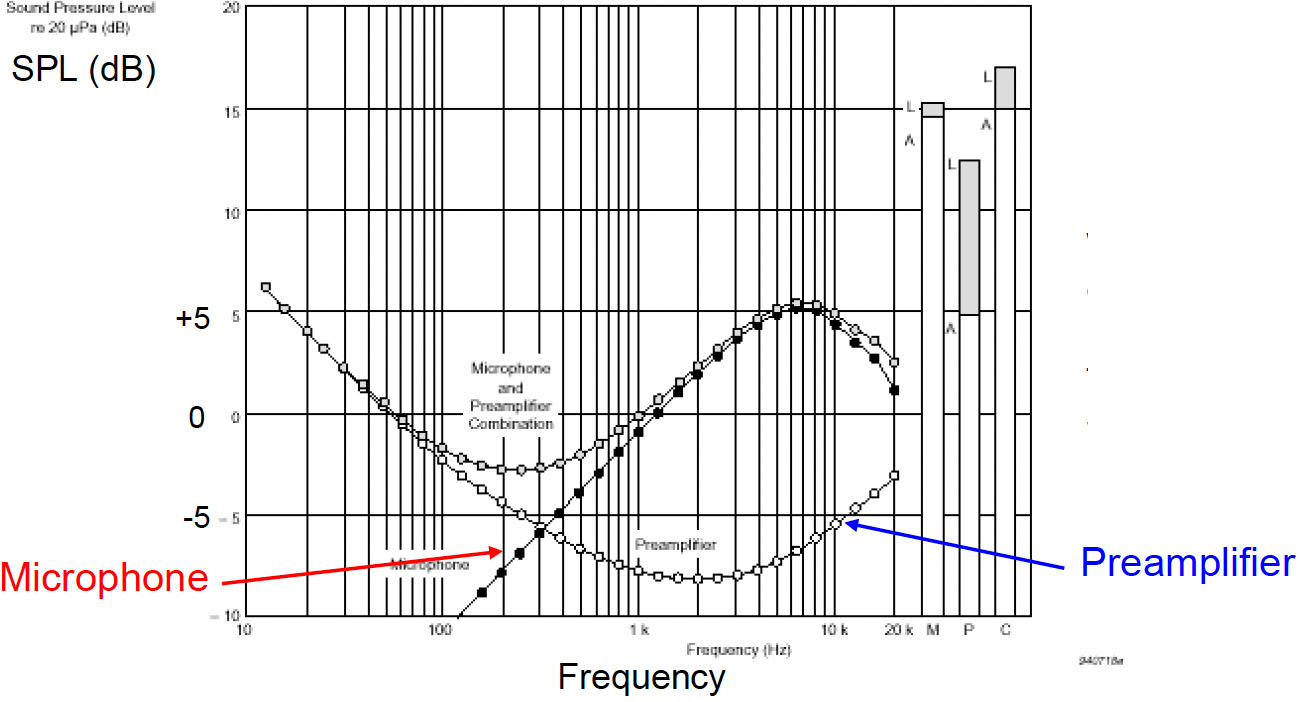
\includegraphics[width=0.75\textwidth]{mic_preamp_noise.png}
    \caption{Third-octave noise spectra of a complete measurement system consisting of a \(\tfrac{1}{2}''\) free-field condenser microphone (\SI{50}{\milli\volt\per\pascal}) and a high-quality preamplifier: preamplifier electronic noise dominates below approximately \SI{1}{\kilo\hertz}, while Brownian motion of the diaphragm sets the limit at high frequencies}
\end{figure}

This crossover behavior has practical design consequences: for low-noise recording of quiet sound sources, a large-diaphragm high-sensitivity capsule reduces the microphone's own noise contribution, while the preamplifier noise floor must be minimized independently; for demanding measurement applications, the sensitivity of the capsule also determines how much preamplifier gain is required, which in turn sets the amplifier's noise contribution referred to the input.

\subsection{Dynamic Range}

The dynamic range of a microphone is the interval between the minimum detectable sound pressure, set by the self-noise floor and the maximum allowable sound pressure, set by the onset of nonlinear distortion at a specified level.
The upper limit is conventionally quoted as the SPL at which the total harmonic distortion (THD) reaches \SI{1}{\percent} or \SI{3}{\percent}:
\[
\text{Dynamic Range} = \mathrm{SPL}_{\mathrm{max}} - \text{Noise level [dB SPL]}
\]
For the Shure KSM9 cited in section \ref{sc:112}, the self-noise is \SI{22}{\decibel SPL} (A-weighted) and the maximum SPL at \SI{1}{\percent} THD is \SI{152}{\decibel SPL}, yielding a dynamic range of \SI{130}{\decibel}.
High-performance measurement microphones can achieve dynamic ranges exceeding \SI{130}{\decibel}, enabling faithful capture of acoustic environments from the quietest anechoic chamber to the loudest aeroacoustic or industrial source without gain switching.
